% TraceAssist pipeline, from question to answer. Standalone; build with
%   pdflatex traceassist_pipeline.tex
% and include the PDF with 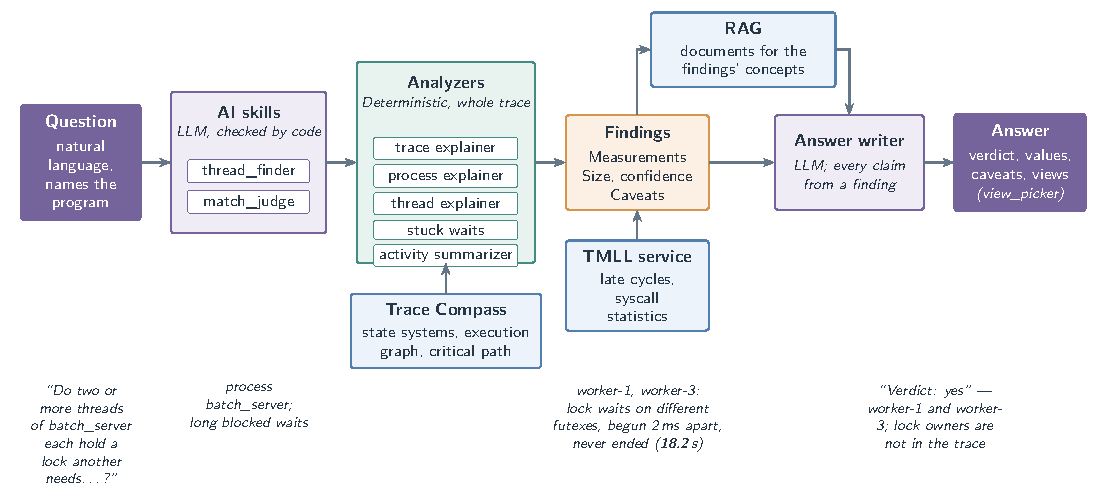
\includegraphics[width=\textwidth]{traceassist_pipeline}.
% Colours follow report/figures/unified_workflow.tex.
\documentclass[tikz,border=2mm]{standalone}
\usepackage[T1]{fontenc}
\usepackage{lmodern}
\usetikzlibrary{arrows.meta,positioning,calc}

\definecolor{ink}{HTML}{273746}
\definecolor{line}{HTML}{657786}
\definecolor{purple}{HTML}{75649C}
\definecolor{teal}{HTML}{428C83}
\definecolor{blue}{HTML}{527FAE}
\definecolor{orange}{HTML}{D5954C}
\definecolor{greenfill}{HTML}{E8F3F0}
\definecolor{bluefill}{HTML}{EDF3FA}
\definecolor{lavender}{HTML}{F0ECF5}
\definecolor{orangefill}{HTML}{FBF0E3}

% Box heading, and the role tag under it.
\newcommand{\hd}[1]{{\bfseries\fontsize{8.5}{10}\selectfont #1}}
\newcommand{\role}[1]{{\itshape\fontsize{7}{8.5}\selectfont #1}}

\begin{document}
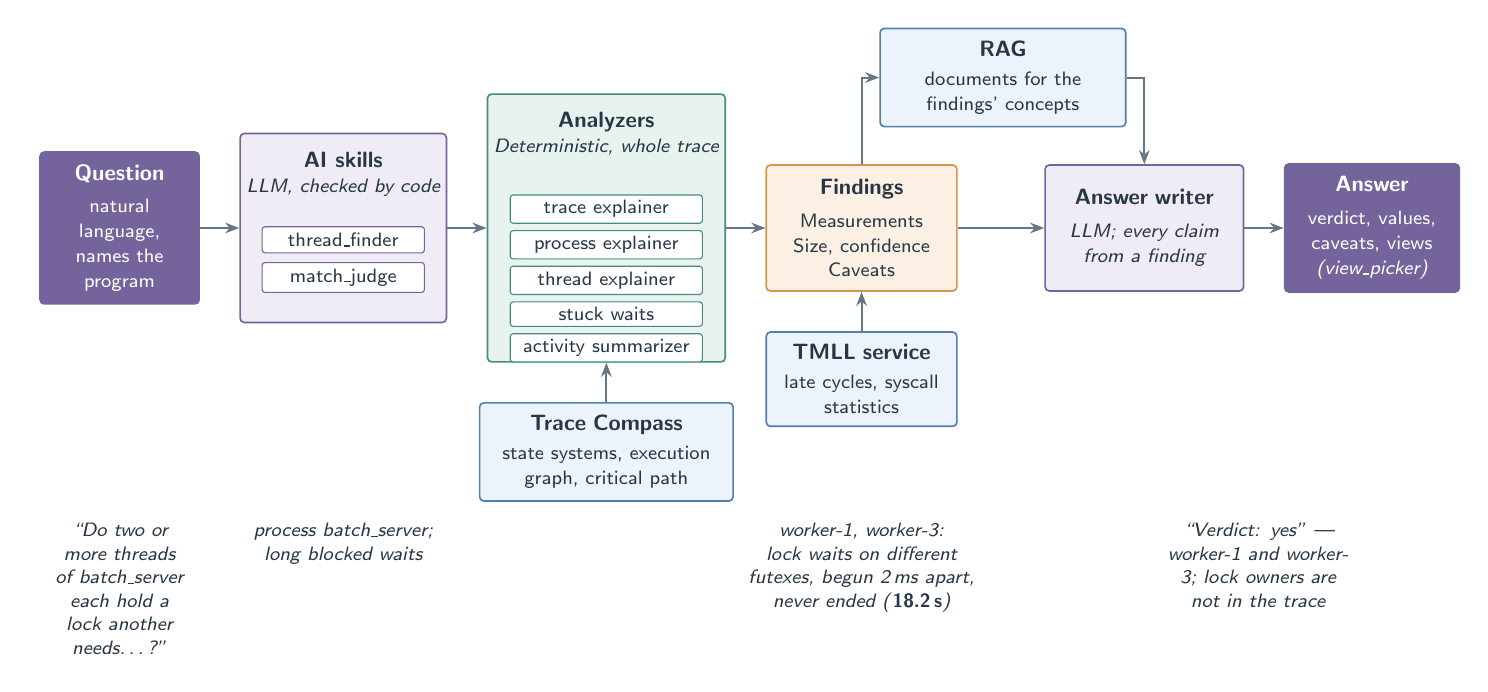
\begin{tikzpicture}[
  font=\sffamily\fontsize{7.5}{9}\selectfont, text=ink,
  box/.style={draw, rounded corners=1.5pt, align=center, inner sep=1.6mm,
              line width=.6pt, minimum height=16mm},
  flow/.style={draw=line, line width=.7pt, -{Stealth[length=1.8mm]}},
  example/.style={font=\sffamily\itshape\fontsize{7}{8.5}\selectfont, text=ink,
                  align=center, text width=#1, anchor=north},
  node distance=5mm and 5mm]

% ---- main flow -----------------------------------------------------------
\node[box, draw=purple, fill=purple, text=white, text width=17mm] (q)
  {\hd{Question}\\[1mm] natural language,\\ names the program};

% AI skills: LLM decisions checked by code.
\node[box, draw=purple, fill=lavender, text width=23mm, right=of q, minimum height=24mm] (sk) {};
\node[anchor=north, align=center] at ($(sk.north)+(0,-1.2mm)$)
  {\hd{AI skills}\\ \role{LLM, checked by code}};
\node[draw=purple, fill=white, rounded corners=1pt, text width=19mm, align=center,
      inner sep=.8mm] (tf) at ($(sk.center)+(0,-1.5mm)$) {thread\_finder};
\node[draw=purple, fill=white, rounded corners=1pt, text width=19mm, align=center,
      inner sep=.8mm, below=1.1mm of tf] (mj) {match\_judge};

% Analyzers.
\node[box, draw=teal, fill=greenfill, text width=27mm, right=of sk,
      minimum height=34mm] (an) {};
\node[anchor=north, align=center] at ($(an.north)+(0,-1.2mm)$)
  {\hd{Analyzers}\\ \role{Deterministic, whole trace}};
\node[draw=teal, fill=white, rounded corners=1pt, text width=23mm, align=center,
      inner sep=.7mm] (te) at ($(an.center)+(0,2.4mm)$) {trace explainer};
\node[draw=teal, fill=white, rounded corners=1pt, text width=23mm, align=center,
      inner sep=.7mm, below=.8mm of te] (pe) {process explainer};
\node[draw=teal, fill=white, rounded corners=1pt, text width=23mm, align=center,
      inner sep=.7mm, below=.8mm of pe] (th) {thread explainer};
\node[draw=teal, fill=white, rounded corners=1pt, text width=23mm, align=center,
      inner sep=.7mm, below=.8mm of th] (sw) {stuck waits};
\node[draw=teal, fill=white, rounded corners=1pt, text width=23mm, align=center,
      inner sep=.7mm, below=.8mm of sw] (as) {activity summarizer};

\node[box, draw=orange, fill=orangefill, text width=21mm, right=of an] (fd)
  {\hd{Findings}\\[1mm] Measurements\\ Size, confidence\\ Caveats};

\node[box, draw=purple, fill=lavender, text width=22mm, right=11mm of fd] (llm)
  {\hd{Answer writer}\\[1mm] \role{LLM; every claim}\\ \role{from a finding}};

\node[box, draw=purple, fill=purple, text=white, text width=19mm, right=of llm] (ans)
  {\hd{Answer}\\[1mm] verdict, values,\\ caveats, views\\ \role{(view\_picker)}};

% ---- inputs, statistics and retrieval -----------------------------------
\node[box, draw=blue, fill=bluefill, text width=29mm, minimum height=10mm,
      below=5mm of an] (tr)
  {\hd{Trace Compass}\\[.5mm] state systems, execution\\ graph, critical path};

\node[box, draw=blue, fill=bluefill, text width=21mm, minimum height=10mm,
      below=5mm of fd] (tmll)
  {\hd{TMLL service}\\[.5mm] late cycles, syscall\\ statistics};

\node[box, draw=blue, fill=bluefill, text width=28mm, minimum height=10mm]
  (rag) at ($(fd.north)!.5!(llm.north)+(0,11mm)$)
  {\hd{RAG}\\[.5mm] documents for the\\ findings' concepts};

% ---- arrows --------------------------------------------------------------
\draw[flow] (q) -- (sk);
\draw[flow] (sk) -- (an);
\draw[flow] (an) -- (fd);
\draw[flow] (fd) -- (llm);
\draw[flow] (llm) -- (ans);
\draw[flow] (tr) -- (an);
\draw[flow] (tmll) -- (fd);
\draw[flow] (fd.north) |- (rag.west);
\draw[flow] (rag.east) -| (llm.north);

% ---- worked example (Q30a, deadlocked batch_server trace) ---------------
\coordinate (ex) at ($(tr.south)+(0,-1.5mm)$);
\node[example=21mm] at (q |- ex)
  {``Do two or more threads of batch\_server each hold a lock another needs\ldots?''};
\node[example=23mm] at (sk |- ex)
  {process batch\_server;\\ long blocked waits};
\node[example=30mm] at (fd |- ex)
  {worker-1, worker-3: lock waits on different futexes, begun 2\,ms apart, never ended (\textbf{18.2\,s})};
\node[example=24mm] at ($(llm |- ex)!.5!(ans |- ex)$)
  {``Verdict: yes'' --- worker-1 and worker-3; lock owners are not in the trace};

\end{tikzpicture}
\end{document}
